\documentclass{standalone}
\begin{document}
	\subsection{Comparison with Manual Annotations}
	
	In order to check the pipeline performances I have compared the  obtained segmentation with the manual annotation. To do that I have considere $5$ scans from the sant'Orsola dataset for which was available also a ground truth. This ground truth consist in an semi-automatic segmentation made with a certified software and refined by an expert with more than $5$ years of experience. After that the segmentation was validated by $5$ experts with at least one year of experience. This segmentation process takes several days. 
	
	In order to compare annotation and pipeline segmentation, I have computed the \emph{sensitivity} and \emph{specificity}: 
	
	\paragraph{Sensitivity} refers to the ability to correctly detect ill areas. It is defined as total number of voxels correctly classified as opacities (True Potitives), over the total number of positives (True Positives + False Negatives) : 
	\begin{equation}\label{eq:sensitivity}
		Sensitivity : \frac{True Positive}{True Positive + False Negatives}
	\end{equation}

	\paragraph{Specificity} relates to the  ability to correctly reject healthy areas. Is defined as the number of rejected pixels(True Negative) against the total number of healthy areas (True Negative + False Positives) : 
	\begin{equation}
		spcificity : \frac{True Negative}{True Negative + False Positives}
	\end{equation}

	I have displayed the results in table\,\ref{tab:Measures}. 
	
		\begin{table}[h!]
		\centering
		\begin{tabular}{|c|c|c|c|c|}
			\hline
			\multirow{2}{*}{}		  & \multicolumn{2}{c|}{Predicted} & \multicolumn{2}{c|}{Annotation} \\ \hline
						& Sensitivity & Specificity	 		& Sensitivity & Specificity		 \\ \hline
			Patient 1	& $0.412$	  &	$\sim 1.00$			&	$0.676$	  &	$ 0.999$ 		 \\ 
			Patient 2	& $0.399$	  & $\sim 1.00$ 		&	$0.698$	  & $ 0.995$		 \\
			Patient 3	& $0.570$	  &	$\sim 1.00$			&	$0.653$	  & $ 0.999$		 \\
			Patient 4	& $0.512$	  & $\sim 1.00$			&	$0.325$	  & $ 0.999$		 \\
			Patient 5 	& $0.628$	  & $\sim 1.00$			&	$0.974$	  &	$ 0.999$		 \\ \hline
		\end{tabular}\caption{Sensitivity and Specificity for the pipeline segmentation and annotation. As a ground truth was used a sem-automatic segmentation made and evaluated by $5$ experts with at least $2$ years of experience.}\label{tab:Measures}
		
	\end{table}

 	The first thing we can notice is that both the method have an high specificity. That means that  they rarely gives positives results for healthy regions (lower type I error rate): means that there is a low probability to obtain false positives. 
 	The situation changes when we consider specificity. We can see that the annotation have achieved a better sensitivity than the pipeline. That means that they rarely gives negative results for GGO regions (lower type II error rate). However this coefficient does not takes into account the rate of false positives, that means we cannot ensure that the detected GGO areas are really sick.
 	
 	This in agreement to the fact that, generally , the operator tends to include large lesion areas. However that is not always the case, since will depends to operator that performs the segmentation.
 	
 	
 	\begin{figure}[h!]
 		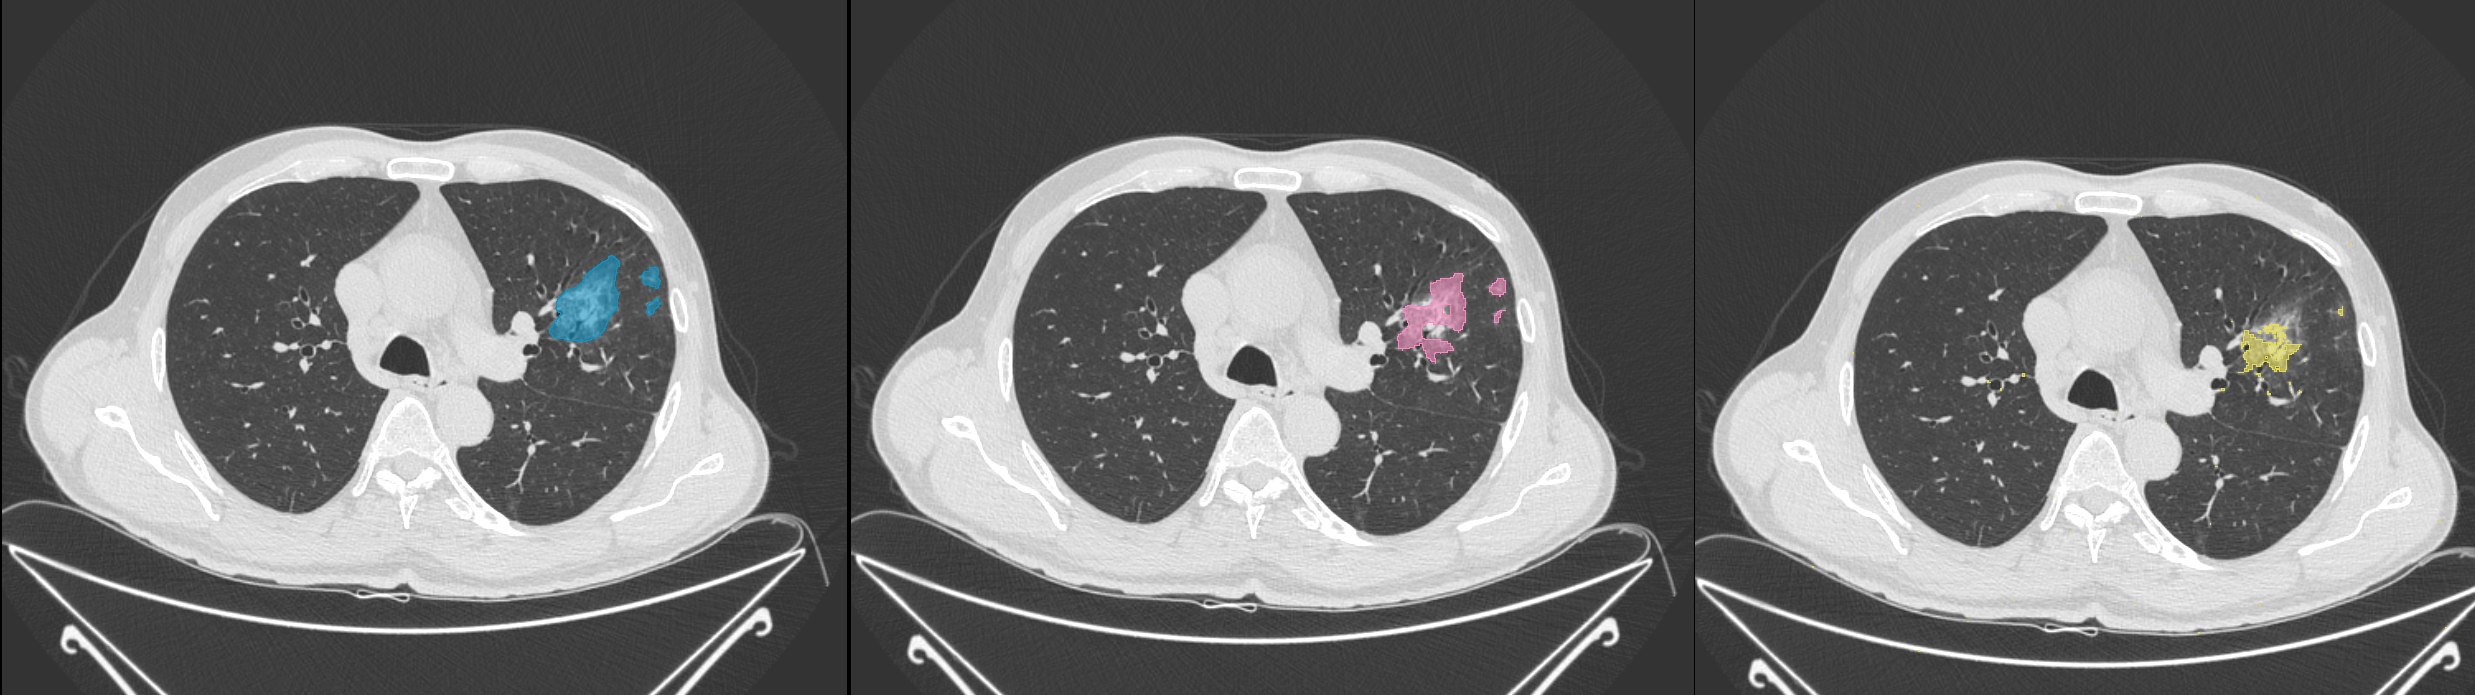
\includegraphics[width=\linewidth, height=.25\textheight]{GTCOM2.png}
 		
 		\caption{Comparison between the ground truth (blue), the pipeline segmentation (pink) and the manual annotation (yellow). We can see that the segmentation obtained by the automatic pipeline is better that the one of the manual annotation.}\label{fig:conf2}
 	\end{figure}
 
 	In \figurename\,\ref{fig:conf2} I have reported the results of the segmentation of Patient $4$. We can see the ground truth (blue), the pipeline segmentation (pink) and the annotation (yellow). In this case we can see that both the pipeline and the annotation correctly identified the lesion areas. However we can see that the annotation is missing a lot of lesion. On the other hand the segmentation achieved by the pipeline seems to cerrectly segment the whole areas. 
 	
 	\begin{figure}[h!]
 		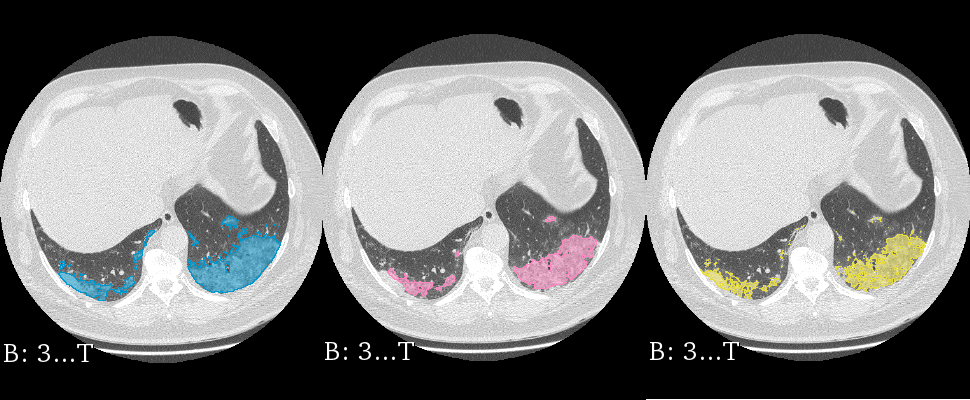
\includegraphics[width=\linewidth]{GTCOMP1.png}
 		
 		\caption{Comparison between the ground truth (blue), the pipeline segmentation (pink) and the manual annotation (yellow). We can see that the GGO an CS areas are correctly identified.}\label{fig:conf1}
 	\end{figure}
 
 	In \figurename\,\ref{fig:conf1} vI have reported the segmentation results for the third patient. We can see the ground truth (blue), the pipeline segmentation (pink) and the annotation (yellow). Also in this case the pipeline seem to correctly identify the opacity. In this case also the annotation seems to be in agreement with the ground truth.
 	
 	\begin{figure}[h!]
 		\centering
 		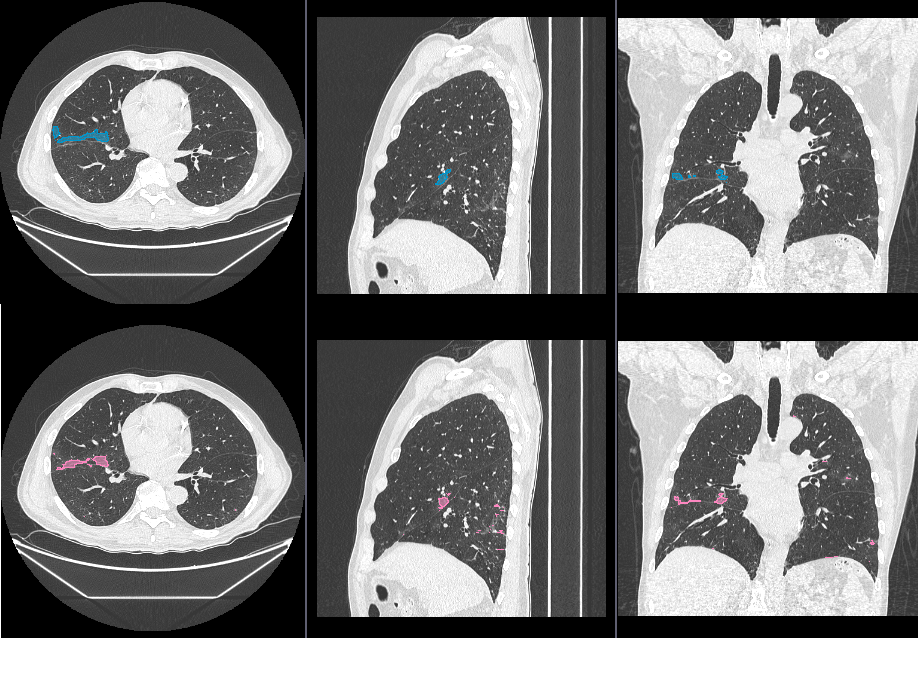
\includegraphics[width=.8\linewidth]{PATIENT1.png}  
 		\caption{Comparison between the gold standard segmentation(blue) and the pipeline results(pink) for axial, sagittal and coronal view of a patient with a low involvement of lung volume. We can see that te main lesion areas are identified, even if an underestimation of the total volume is present together with some small misclassified points.}\label{fig:pat1}
 	\end{figure}
 	
 	Up to now I have considered only two case in which the GGO and CS regions are well defined with high contrast respect to healthy lung volume. In \figurename\,\ref{fig:pat1} I have reported axial, sagittal and coronal view of the ground truth (blue) and pipeline segmentation (pink) for the first patient. This patient presents a low volume of GGO and CS. Moreover the identification is difficult due to the low contrast between lesion areas healthy lung volume. As we can see the lesion areas are correctly identified even if some misclassified regions are presents. 
 	
 	In the end I have to point out that the annotation and ground truth, since are obtained by semi-automatic method, requires  trained personnel and several hours (the first) or days (the seconds).  
 	
	

\end{document}